\section{Datasets}
\label{sec:datasets}



We obtained a snapshot of LN on 2020-02-25 from \url{https://ln.bigsun.xyz} and parsed with the (anonymized) scripts available at~\cite{Tikhomirov2019}.
%\footnote{Our experiments are based on data from \url{https://ln.bigsun.xyz/}.
%	The (anonymized) scripts are available at~\cite{LightningPrivacy}.}
This snapshot consists of $5929$~nodes and $35233$~channels.
We model this data as an undirected multi-graph (i.e., may contain multiple edges between each pair of nodes), 
representing the fact that several channels can be shared by two LN nodes.
We only considered the largest connected component, 
which contains $5862$~nodes $(98.87\%)$ and $35196$~channels $(99.89\%)$.
We observe that this subgraph contains a representative sample of the LN.
We refer to this dataset as \emph{LN20}.

Based on \emph{LN20}, 
LN nodes have an average degree of $12.01$ and a median degree of $3$ (see~\cref{fig:node-degree-histogram,fig:channel-capacity-histogram}).
The majority of nodes have very few channels, 
whereas there is a small number of nodes with many channels. 
In particular, there are more than 1744 nodes with degree 1, and the most connected node has 1198~channels.
The capacity is also unequally distributed.
 %\footnote{Public key \texttt{03ffdd7fd4656a55a63a4b6e154325859681718ba2fac40e51cb61752506bb8c7b}.}
These observations motivate the methodology in our experiments in~\cref{sec:sec-priv-attacks}. 

We also derive a series of historic snapshots which represent the state of LN on the first day of each month from April~2018 to February~2020.
We refer to this dataset as \textit{LNHist} 
and use it in our study of concurrent payments on LN performance over time (\cref{sec:attack}).
%See Appendix~\ref{sec:historic} for our study of the temporal evolution of the LN based on LNHist.


\begin{figure}[tb]
	\centering
	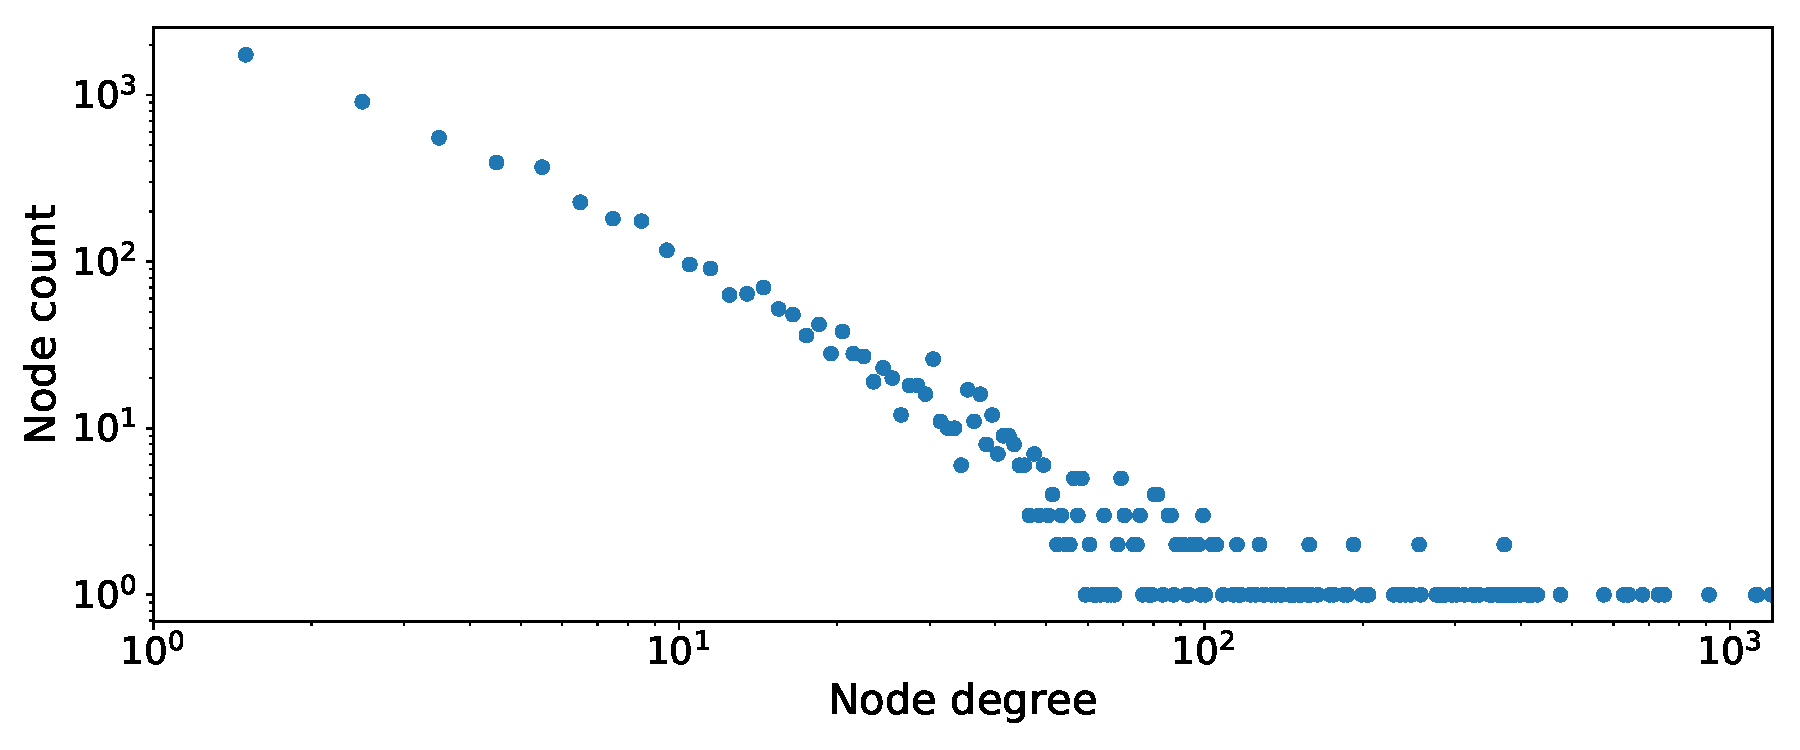
\includegraphics[width=\columnwidth]{node-degree-histogram}
	\caption{Node degree distribution.\label{fig:node-degree-histogram}}
\end{figure}

\begin{figure}[tb]
	\centering
	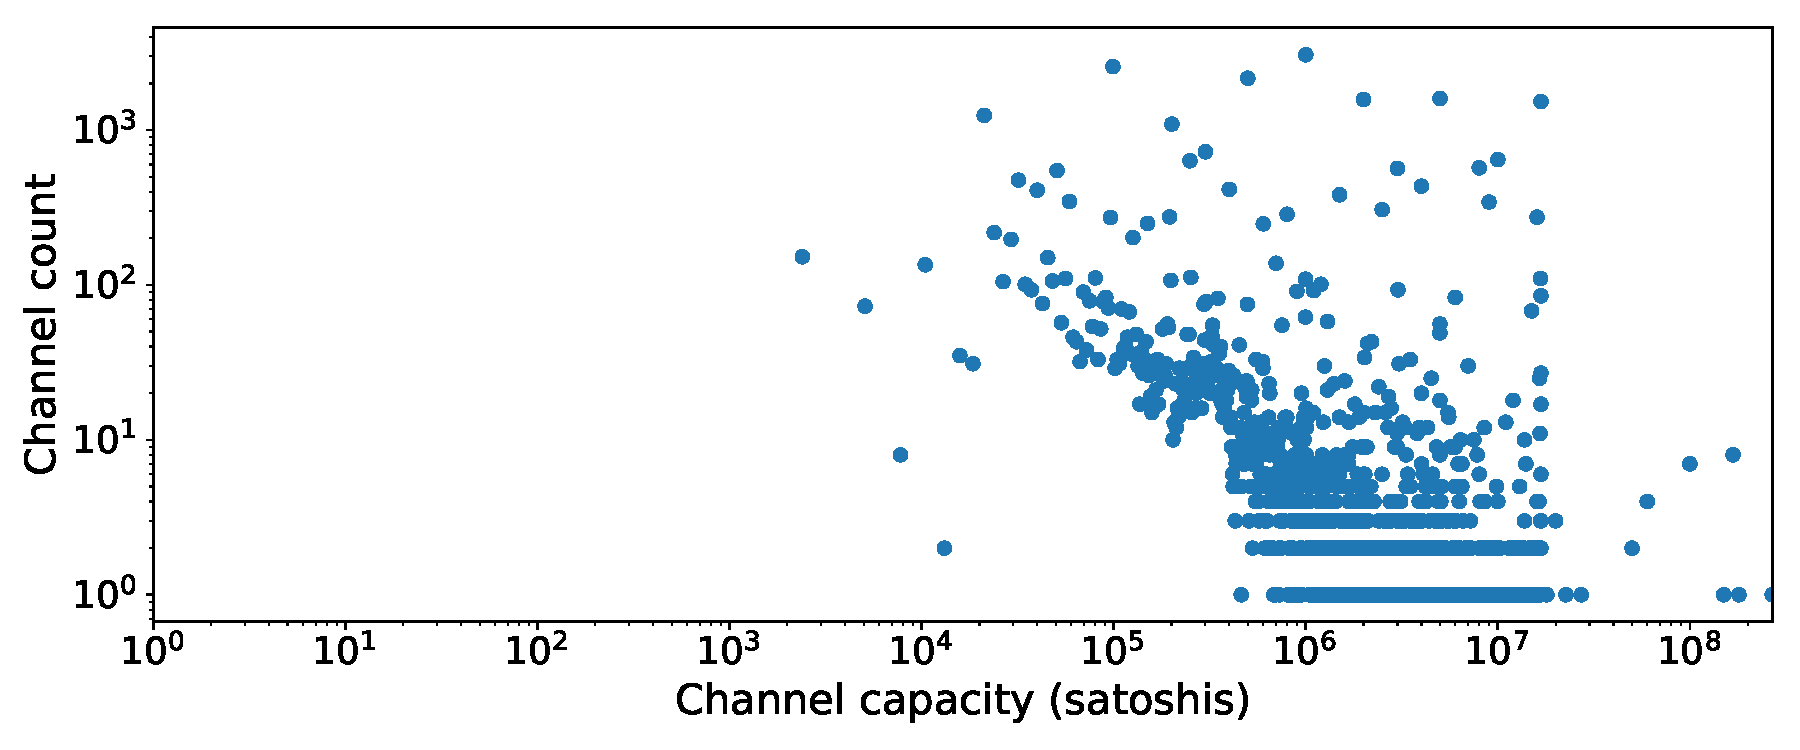
\includegraphics[width=\columnwidth]{channel-capacity-histogram}
	\caption{Channel capacity distribution.\label{fig:channel-capacity-histogram}}
\end{figure}

\subsubsection*{Ethical considerations} 
Our analysis is based solely on publicly available data. 
We do not interfere with the LN activity, nor deanonymize any of its nodes. 
